\documentclass[1p]{elsarticle_modified}
%\bibliographystyle{elsarticle-num}

%\usepackage[colorlinks]{hyperref}
%\usepackage{abbrmath_seonhwa} %\Abb, \Ascr, \Acal ,\Abf, \Afrak
\usepackage{amsfonts}
\usepackage{amssymb}
\usepackage{amsmath}
\usepackage{amsthm}
\usepackage{scalefnt}
\usepackage{amsbsy}
\usepackage{kotex}
\usepackage{caption}
\usepackage{subfig}
\usepackage{color}
\usepackage{graphicx}
\usepackage{xcolor} %% white, black, red, green, blue, cyan, magenta, yellow
\usepackage{float}
\usepackage{setspace}
\usepackage{hyperref}

\usepackage{tikz}
\usetikzlibrary{arrows}

\usepackage{multirow}
\usepackage{array} % fixed length table
\usepackage{hhline}

%%%%%%%%%%%%%%%%%%%%%
\makeatletter
\renewcommand*\env@matrix[1][\arraystretch]{%
	\edef\arraystretch{#1}%
	\hskip -\arraycolsep
	\let\@ifnextchar\new@ifnextchar
	\array{*\c@MaxMatrixCols c}}
\makeatother %https://tex.stackexchange.com/questions/14071/how-can-i-increase-the-line-spacing-in-a-matrix
%%%%%%%%%%%%%%%

\usepackage[normalem]{ulem}

\newcommand{\msout}[1]{\ifmmode\text{\sout{\ensuremath{#1}}}\else\sout{#1}\fi}
%SOURCE: \msout is \stkout macro in https://tex.stackexchange.com/questions/20609/strikeout-in-math-mode

\newcommand{\cancel}[1]{
	\ifmmode
	{\color{red}\msout{#1}}
	\else
	{\color{red}\sout{#1}}
	\fi
}

\newcommand{\add}[1]{
	{\color{blue}\uwave{#1}}
}

\newcommand{\replace}[2]{
	\ifmmode
	{\color{red}\msout{#1}}{\color{blue}\uwave{#2}}
	\else
	{\color{red}\sout{#1}}{\color{blue}\uwave{#2}}
	\fi
}

\newcommand{\Sol}{\mathcal{S}} %segment
\newcommand{\D}{D} %diagram
\newcommand{\A}{\mathcal{A}} %arc


%%%%%%%%%%%%%%%%%%%%%%%%%%%%%5 test

\def\sl{\operatorname{\textup{SL}}(2,\Cbb)}
\def\psl{\operatorname{\textup{PSL}}(2,\Cbb)}
\def\quan{\mkern 1mu \triangleright \mkern 1mu}

\theoremstyle{definition}
\newtheorem{thm}{Theorem}[section]
\newtheorem{prop}[thm]{Proposition}
\newtheorem{lem}[thm]{Lemma}
\newtheorem{ques}[thm]{Question}
\newtheorem{cor}[thm]{Corollary}
\newtheorem{defn}[thm]{Definition}
\newtheorem{exam}[thm]{Example}
\newtheorem{rmk}[thm]{Remark}
\newtheorem{alg}[thm]{Algorithm}

\newcommand{\I}{\sqrt{-1}}
\begin{document}

%\begin{frontmatter}
%
%\title{Boundary parabolic representations of knots up to 8 crossings}
%
%%% Group authors per affiliation:
%\author{Yunhi Cho} 
%\address{Department of Mathematics, University of Seoul, Seoul, Korea}
%\ead{yhcho@uos.ac.kr}
%
%
%\author{Seonhwa Kim} %\fnref{s_kim}}
%\address{Center for Geometry and Physics, Institute for Basic Science, Pohang, 37673, Korea}
%\ead{ryeona17@ibs.re.kr}
%
%\author{Hyuk Kim}
%\address{Department of Mathematical Sciences, Seoul National University, Seoul 08826, Korea}
%\ead{hyukkim@snu.ac.kr}
%
%\author{Seokbeom Yoon}
%\address{Department of Mathematical Sciences, Seoul National University, Seoul, 08826,  Korea}
%\ead{sbyoon15@snu.ac.kr}
%
%\begin{abstract}
%We find all boundary parabolic representation of knots up to 8 crossings.
%
%\end{abstract}
%\begin{keyword}
%    \MSC[2010] 57M25 
%\end{keyword}
%
%\end{frontmatter}

%\linenumbers
%\tableofcontents
%
\newcommand\colored[1]{\textcolor{white}{\rule[-0.35ex]{0.8em}{1.4ex}}\kern-0.8em\color{red} #1}%
%\newcommand\colored[1]{\textcolor{white}{ #1}\kern-2.17ex	\textcolor{white}{ #1}\kern-1.81ex	\textcolor{white}{ #1}\kern-2.15ex\color{red}#1	}

{\Large $\underline{12a_{0269}~(K12a_{0269})}$}

\setlength{\tabcolsep}{10pt}
\renewcommand{\arraystretch}{1.6}
\vspace{1cm}\begin{tabular}{m{100pt}>{\centering\arraybackslash}m{274pt}}
\multirow{5}{120pt}{
	\centering
	\includegraphics[width=112pt]{../../../GIT/diagram.site/Diagrams/png/1070_12a_0269.png}\\
\ \ \ A knot diagram\footnotemark}&
\allowdisplaybreaks
\textbf{Linearized knot diagam} \\
\cline{2-2}
 &
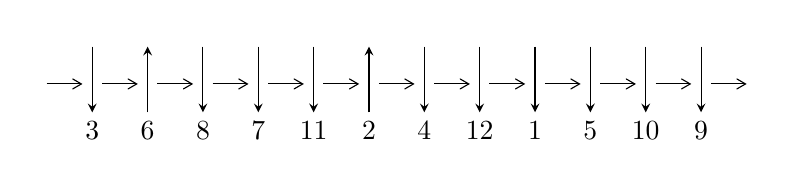
\begin{tikzpicture}[x=20pt, y=17pt]
	% nodes
	\node (C0) at (0, 0) {};
	\node (C1) at (1, 0) {};
	\node (C1U) at (1, +1) {};
	\node (C1D) at (1, -1) {3};

	\node (C2) at (2, 0) {};
	\node (C2U) at (2, +1) {};
	\node (C2D) at (2, -1) {6};

	\node (C3) at (3, 0) {};
	\node (C3U) at (3, +1) {};
	\node (C3D) at (3, -1) {8};

	\node (C4) at (4, 0) {};
	\node (C4U) at (4, +1) {};
	\node (C4D) at (4, -1) {7};

	\node (C5) at (5, 0) {};
	\node (C5U) at (5, +1) {};
	\node (C5D) at (5, -1) {11};

	\node (C6) at (6, 0) {};
	\node (C6U) at (6, +1) {};
	\node (C6D) at (6, -1) {2};

	\node (C7) at (7, 0) {};
	\node (C7U) at (7, +1) {};
	\node (C7D) at (7, -1) {4};

	\node (C8) at (8, 0) {};
	\node (C8U) at (8, +1) {};
	\node (C8D) at (8, -1) {12};

	\node (C9) at (9, 0) {};
	\node (C9U) at (9, +1) {};
	\node (C9D) at (9, -1) {1};

	\node (C10) at (10, 0) {};
	\node (C10U) at (10, +1) {};
	\node (C10D) at (10, -1) {5};

	\node (C11) at (11, 0) {};
	\node (C11U) at (11, +1) {};
	\node (C11D) at (11, -1) {10};

	\node (C12) at (12, 0) {};
	\node (C12U) at (12, +1) {};
	\node (C12D) at (12, -1) {9};
	\node (C13) at (13, 0) {};

	% arrows
	\draw[->,>={angle 60}]
	(C0) edge (C1) (C1) edge (C2) (C2) edge (C3) (C3) edge (C4) (C4) edge (C5) (C5) edge (C6) (C6) edge (C7) (C7) edge (C8) (C8) edge (C9) (C9) edge (C10) (C10) edge (C11) (C11) edge (C12) (C12) edge (C13) ;	\draw[->,>=stealth]
	(C1U) edge (C1D) (C2D) edge (C2U) (C3U) edge (C3D) (C4U) edge (C4D) (C5U) edge (C5D) (C6D) edge (C6U) (C7U) edge (C7D) (C8U) edge (C8D) (C9U) edge (C9D) (C10U) edge (C10D) (C11U) edge (C11D) (C12U) edge (C12D) ;
	\end{tikzpicture} \\
\hhline{~~} \\& 
\textbf{Solving Sequence} \\ \cline{2-2} 
 &
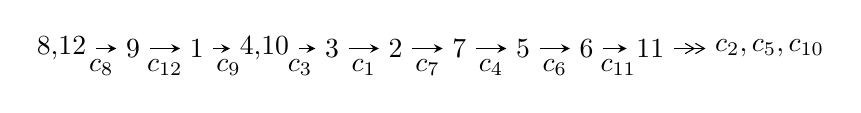
\begin{tikzpicture}[x=23pt, y=7pt]
	% node
	\node (A0) at (-1/8, 0) {8,12};
	\node (A1) at (1, 0) {9};
	\node (A2) at (2, 0) {1};
	\node (A3) at (49/16, 0) {4,10};
	\node (A4) at (33/8, 0) {3};
	\node (A5) at (41/8, 0) {2};
	\node (A6) at (49/8, 0) {7};
	\node (A7) at (57/8, 0) {5};
	\node (A8) at (65/8, 0) {6};
	\node (A9) at (73/8, 0) {11};
	\node (C1) at (1/2, -1) {$c_{8}$};
	\node (C2) at (3/2, -1) {$c_{12}$};
	\node (C3) at (5/2, -1) {$c_{9}$};
	\node (C4) at (29/8, -1) {$c_{3}$};
	\node (C5) at (37/8, -1) {$c_{1}$};
	\node (C6) at (45/8, -1) {$c_{7}$};
	\node (C7) at (53/8, -1) {$c_{4}$};
	\node (C8) at (61/8, -1) {$c_{6}$};
	\node (C9) at (69/8, -1) {$c_{11}$};
	\node (A10) at (11, 0) {$c_{2},c_{5},c_{10}$};

	% edge
	\draw[->,>=stealth]	
	(A0) edge (A1) (A1) edge (A2) (A2) edge (A3) (A3) edge (A4) (A4) edge (A5) (A5) edge (A6) (A6) edge (A7) (A7) edge (A8) (A8) edge (A9) ;
	\draw[->>,>={angle 60}]	
	(A9) edge (A10);
\end{tikzpicture} \\ 

\end{tabular} \\

\footnotetext{
The image of knot diagram is generated by the software ``\textbf{Draw programme}" developed by Andrew Bartholomew(\url{http://www.layer8.co.uk/maths/draw/index.htm\#Running-draw}), where we modified some parts for our purpose(\url{https://github.com/CATsTAILs/LinksPainter}).
}\phantom \\ \newline 
\centering \textbf{Ideals for irreducible components\footnotemark of $X_{\text{par}}$} 
 
\begin{align*}
I^u_{1}&=\langle 
-8.62713\times10^{15} u^{65}-2.11985\times10^{16} u^{64}+\cdots+2.49267\times10^{16} b-1.13014\times10^{15},\\
\phantom{I^u_{1}}&\phantom{= \langle  }4.31598\times10^{16} u^{65}+1.40820\times10^{17} u^{64}+\cdots+9.97068\times10^{16} a+5.56705\times10^{17},\;u^{66}+4 u^{65}+\cdots+35 u+4\rangle \\
I^u_{2}&=\langle 
-83 u^7 a^2-105 u^7 a+\cdots-2 a+166,\;-2 u^7 a^2+8 u^7 a+\cdots+18 a-6,\\
\phantom{I^u_{2}}&\phantom{= \langle  }u^8+u^7-3 u^6-2 u^5+3 u^4+2 u-1\rangle \\
I^u_{3}&=\langle 
- u^4 a+u^2 a+u^3- a u+b+a- u+1,\;u^4-2 u^2 a+u^3+a^2-2 a u-2 u^2+2 a+3,\\
\phantom{I^u_{3}}&\phantom{= \langle  }u^5+u^4-2 u^3- u^2+u-1\rangle \\
I^u_{4}&=\langle 
-2 a^3- a^2+b- a,\;2 a^4+3 a^3+4 a^2+3 a+1,\;u-1\rangle \\
\\
\end{align*}
\raggedright * 4 irreducible components of $\dim_{\mathbb{C}}=0$, with total 104 representations.\\
\footnotetext{All coefficients of polynomials are rational numbers. But the coefficients are sometimes approximated in decimal forms when there is not enough margin.}
\newpage
\renewcommand{\arraystretch}{1}
\centering \section*{I. $I^u_{1}= \langle -8.63\times10^{15} u^{65}-2.12\times10^{16} u^{64}+\cdots+2.49\times10^{16} b-1.13\times10^{15},\;4.32\times10^{16} u^{65}+1.41\times10^{17} u^{64}+\cdots+9.97\times10^{16} a+5.57\times10^{17},\;u^{66}+4 u^{65}+\cdots+35 u+4 \rangle$}
\flushleft \textbf{(i) Arc colorings}\\
\begin{tabular}{m{7pt} m{180pt} m{7pt} m{180pt} }
\flushright $a_{8}=$&$\begin{pmatrix}1\\0\end{pmatrix}$ \\
\flushright $a_{12}=$&$\begin{pmatrix}0\\u\end{pmatrix}$ \\
\flushright $a_{9}=$&$\begin{pmatrix}1\\u^2\end{pmatrix}$ \\
\flushright $a_{1}=$&$\begin{pmatrix}- u\\- u^3+u\end{pmatrix}$ \\
\flushright $a_{4}=$&$\begin{pmatrix}-0.432868 u^{65}-1.41234 u^{64}+\cdots-25.5775 u-5.58342\\0.346100 u^{65}+0.850432 u^{64}+\cdots+4.81724 u+0.0453386\end{pmatrix}$ \\
\flushright $a_{10}=$&$\begin{pmatrix}- u^2+1\\- u^4+2 u^2\end{pmatrix}$ \\
\flushright $a_{3}=$&$\begin{pmatrix}-0.0867675 u^{65}-0.561913 u^{64}+\cdots-20.7603 u-5.53808\\0.346100 u^{65}+0.850432 u^{64}+\cdots+4.81724 u+0.0453386\end{pmatrix}$ \\
\flushright $a_{2}=$&$\begin{pmatrix}-0.00547462 u^{65}+0.184155 u^{64}+\cdots+13.3969 u+1.98843\\-0.0754890 u^{65}-0.133427 u^{64}+\cdots+1.98495 u+0.305099\end{pmatrix}$ \\
\flushright $a_{7}=$&$\begin{pmatrix}-0.132128 u^{65}-0.450532 u^{64}+\cdots-13.0108 u-0.408261\\0.468288 u^{65}+1.18384 u^{64}+\cdots+9.40368 u+1.08447\end{pmatrix}$ \\
\flushright $a_{5}=$&$\begin{pmatrix}-0.410233 u^{65}-1.26602 u^{64}+\cdots-24.2954 u-3.94259\\0.275978 u^{65}+0.641853 u^{64}+\cdots+2.90510 u-0.110199\end{pmatrix}$ \\
\flushright $a_{6}=$&$\begin{pmatrix}-0.114697 u^{65}-0.539674 u^{64}+\cdots-18.9899 u-3.33232\\0.265315 u^{65}+0.589033 u^{64}+\cdots+2.64364 u-0.213478\end{pmatrix}$ \\
\flushright $a_{11}=$&$\begin{pmatrix}u^5-2 u^3+u\\u^7-3 u^5+2 u^3+u\end{pmatrix}$\\&\end{tabular}
\flushleft \textbf{(ii) Obstruction class $= -1$}\\~\\
\flushleft \textbf{(iii) Cusp Shapes $= -\frac{22848277210974797}{49853400611938144} u^{65}-\frac{33245267932303681}{49853400611938144} u^{64}+\cdots+\frac{1408726762689068359}{49853400611938144} u+\frac{18620167407452593}{12463350152984536}$}\\~\\
\newpage\renewcommand{\arraystretch}{1}
\flushleft \textbf{(iv) u-Polynomials at the component}\newline \\
\begin{tabular}{m{50pt}|m{274pt}}
Crossings & \hspace{64pt}u-Polynomials at each crossing \\
\hline $$\begin{aligned}c_{1}\end{aligned}$$&$\begin{aligned}
&u^{66}+24 u^{65}+\cdots+5878 u+289
\end{aligned}$\\
\hline $$\begin{aligned}c_{2},c_{6}\end{aligned}$$&$\begin{aligned}
&u^{66}-2 u^{65}+\cdots-138 u+17
\end{aligned}$\\
\hline $$\begin{aligned}c_{3},c_{4},c_{7}\end{aligned}$$&$\begin{aligned}
&u^{66}-2 u^{65}+\cdots-186 u+17
\end{aligned}$\\
\hline $$\begin{aligned}c_{5},c_{10}\end{aligned}$$&$\begin{aligned}
&u^{66}-2 u^{65}+\cdots-16 u+64
\end{aligned}$\\
\hline $$\begin{aligned}c_{8},c_{9},c_{12}\end{aligned}$$&$\begin{aligned}
&u^{66}-4 u^{65}+\cdots-35 u+4
\end{aligned}$\\
\hline $$\begin{aligned}c_{11}\end{aligned}$$&$\begin{aligned}
&u^{66}+24 u^{65}+\cdots-13056 u+4096
\end{aligned}$\\
\hline
\end{tabular}\\~\\
\newpage\renewcommand{\arraystretch}{1}
\flushleft \textbf{(v) Riley Polynomials at the component}\newline \\
\begin{tabular}{m{50pt}|m{274pt}}
Crossings & \hspace{64pt}Riley Polynomials at each crossing \\
\hline $$\begin{aligned}c_{1}\end{aligned}$$&$\begin{aligned}
&y^{66}+48 y^{65}+\cdots+10918642 y+83521
\end{aligned}$\\
\hline $$\begin{aligned}c_{2},c_{6}\end{aligned}$$&$\begin{aligned}
&y^{66}+24 y^{65}+\cdots+5878 y+289
\end{aligned}$\\
\hline $$\begin{aligned}c_{3},c_{4},c_{7}\end{aligned}$$&$\begin{aligned}
&y^{66}+72 y^{65}+\cdots-9674 y+289
\end{aligned}$\\
\hline $$\begin{aligned}c_{5},c_{10}\end{aligned}$$&$\begin{aligned}
&y^{66}-24 y^{65}+\cdots+13056 y+4096
\end{aligned}$\\
\hline $$\begin{aligned}c_{8},c_{9},c_{12}\end{aligned}$$&$\begin{aligned}
&y^{66}-56 y^{65}+\cdots-657 y+16
\end{aligned}$\\
\hline $$\begin{aligned}c_{11}\end{aligned}$$&$\begin{aligned}
&y^{66}+28 y^{65}+\cdots-578879488 y+16777216
\end{aligned}$\\
\hline
\end{tabular}\\~\\
\newpage\flushleft \textbf{(vi) Complex Volumes and Cusp Shapes}
$$\begin{array}{c|c|c}  
\text{Solutions to }I^u_{1}& \I (\text{vol} + \sqrt{-1}CS) & \text{Cusp shape}\\
 \hline 
\begin{aligned}
u &= \phantom{-}0.667544 + 0.679084 I \\
a &= \phantom{-}0.86928 - 1.38453 I \\
b &= \phantom{-}0.149820 + 1.369760 I\end{aligned}
 & \phantom{-}1.68392 - 4.80194 I & -8.00000 + 6.16806 I \\ \hline\begin{aligned}
u &= \phantom{-}0.667544 - 0.679084 I \\
a &= \phantom{-}0.86928 + 1.38453 I \\
b &= \phantom{-}0.149820 - 1.369760 I\end{aligned}
 & \phantom{-}1.68392 + 4.80194 I & -8.00000 - 6.16806 I \\ \hline\begin{aligned}
u &= \phantom{-}0.189066 + 0.903983 I \\
a &= \phantom{-}0.74953 - 2.41334 I \\
b &= \phantom{-}0.32275 + 1.48528 I\end{aligned}
 & \phantom{-}6.85220 - 11.84780 I & -4.90258 + 7.91039 I \\ \hline\begin{aligned}
u &= \phantom{-}0.189066 - 0.903983 I \\
a &= \phantom{-}0.74953 + 2.41334 I \\
b &= \phantom{-}0.32275 - 1.48528 I\end{aligned}
 & \phantom{-}6.85220 + 11.84780 I & -4.90258 - 7.91039 I \\ \hline\begin{aligned}
u &= \phantom{-}1.083740 + 0.168606 I \\
a &= \phantom{-}1.242980 + 0.094384 I \\
b &= \phantom{-}0.111698 + 0.687804 I\end{aligned}
 & -1.18380 - 0.83133 I & \phantom{-0.000000 } 0 \\ \hline\begin{aligned}
u &= \phantom{-}1.083740 - 0.168606 I \\
a &= \phantom{-}1.242980 - 0.094384 I \\
b &= \phantom{-}0.111698 - 0.687804 I\end{aligned}
 & -1.18380 + 0.83133 I & \phantom{-0.000000 } 0 \\ \hline\begin{aligned}
u &= \phantom{-}0.514125 + 0.739694 I \\
a &= -0.64446 + 1.40518 I \\
b &= \phantom{-}0.065420 - 1.343790 I\end{aligned}
 & \phantom{-}2.12892 - 0.16897 I & -6.25009 + 0.21372 I \\ \hline\begin{aligned}
u &= \phantom{-}0.514125 - 0.739694 I \\
a &= -0.64446 - 1.40518 I \\
b &= \phantom{-}0.065420 + 1.343790 I\end{aligned}
 & \phantom{-}2.12892 + 0.16897 I & -6.25009 - 0.21372 I \\ \hline\begin{aligned}
u &= \phantom{-}0.130215 + 0.881989 I \\
a &= -0.46791 + 2.65814 I \\
b &= -0.21538 - 1.51295 I\end{aligned}
 & \phantom{-}8.94622 - 5.72427 I & -2.18443 + 3.66030 I \\ \hline\begin{aligned}
u &= \phantom{-}0.130215 - 0.881989 I \\
a &= -0.46791 - 2.65814 I \\
b &= -0.21538 + 1.51295 I\end{aligned}
 & \phantom{-}8.94622 + 5.72427 I & -2.18443 - 3.66030 I\\
 \hline 
 \end{array}$$\newpage$$\begin{array}{c|c|c}  
\text{Solutions to }I^u_{1}& \I (\text{vol} + \sqrt{-1}CS) & \text{Cusp shape}\\
 \hline 
\begin{aligned}
u &= \phantom{-}1.046270 + 0.417779 I \\
a &= -0.002021 - 0.327101 I \\
b &= \phantom{-}0.730735 - 0.378556 I\end{aligned}
 & -1.82882 + 3.10174 I & \phantom{-0.000000 } 0 \\ \hline\begin{aligned}
u &= \phantom{-}1.046270 - 0.417779 I \\
a &= -0.002021 + 0.327101 I \\
b &= \phantom{-}0.730735 + 0.378556 I\end{aligned}
 & -1.82882 - 3.10174 I & \phantom{-0.000000 } 0 \\ \hline\begin{aligned}
u &= \phantom{-}0.173783 + 0.831807 I \\
a &= -0.307675 - 0.785989 I \\
b &= \phantom{-}0.845661 + 0.377568 I\end{aligned}
 & \phantom{-}0.84572 - 7.60212 I & -7.64898 + 8.09357 I \\ \hline\begin{aligned}
u &= \phantom{-}0.173783 - 0.831807 I \\
a &= -0.307675 + 0.785989 I \\
b &= \phantom{-}0.845661 - 0.377568 I\end{aligned}
 & \phantom{-}0.84572 + 7.60212 I & -7.64898 - 8.09357 I \\ \hline\begin{aligned}
u &= -1.147790 + 0.229735 I \\
a &= \phantom{-}0.102586 + 1.241460 I \\
b &= -0.19773 - 1.58186 I\end{aligned}
 & \phantom{-}5.40538 - 2.32156 I & \phantom{-0.000000 } 0 \\ \hline\begin{aligned}
u &= -1.147790 - 0.229735 I \\
a &= \phantom{-}0.102586 - 1.241460 I \\
b &= -0.19773 + 1.58186 I\end{aligned}
 & \phantom{-}5.40538 + 2.32156 I & \phantom{-0.000000 } 0 \\ \hline\begin{aligned}
u &= \phantom{-}0.651446 + 0.470027 I \\
a &= \phantom{-}0.284563 + 0.188739 I \\
b &= \phantom{-}0.505053 + 0.174111 I\end{aligned}
 & -3.20898 - 2.48763 I & -16.3622 + 5.4337 I \\ \hline\begin{aligned}
u &= \phantom{-}0.651446 - 0.470027 I \\
a &= \phantom{-}0.284563 - 0.188739 I \\
b &= \phantom{-}0.505053 - 0.174111 I\end{aligned}
 & -3.20898 + 2.48763 I & -16.3622 - 5.4337 I \\ \hline\begin{aligned}
u &= \phantom{-}1.081520 + 0.529987 I \\
a &= -0.355349 + 1.221180 I \\
b &= \phantom{-}0.27716 - 1.46865 I\end{aligned}
 & \phantom{-}4.13434 + 6.78830 I & \phantom{-0.000000 } 0 \\ \hline\begin{aligned}
u &= \phantom{-}1.081520 - 0.529987 I \\
a &= -0.355349 - 1.221180 I \\
b &= \phantom{-}0.27716 + 1.46865 I\end{aligned}
 & \phantom{-}4.13434 - 6.78830 I & \phantom{-0.000000 } 0\\
 \hline 
 \end{array}$$\newpage$$\begin{array}{c|c|c}  
\text{Solutions to }I^u_{1}& \I (\text{vol} + \sqrt{-1}CS) & \text{Cusp shape}\\
 \hline 
\begin{aligned}
u &= -0.071965 + 0.786913 I \\
a &= \phantom{-}0.79882 + 2.76845 I \\
b &= \phantom{-}0.13150 - 1.53519 I\end{aligned}
 & \phantom{-}9.78957 - 0.29681 I & -0.83343 + 1.63973 I \\ \hline\begin{aligned}
u &= -0.071965 - 0.786913 I \\
a &= \phantom{-}0.79882 - 2.76845 I \\
b &= \phantom{-}0.13150 + 1.53519 I\end{aligned}
 & \phantom{-}9.78957 + 0.29681 I & -0.83343 - 1.63973 I \\ \hline\begin{aligned}
u &= \phantom{-}1.143660 + 0.471596 I \\
a &= \phantom{-}0.69893 - 1.38761 I \\
b &= -0.15146 + 1.48688 I\end{aligned}
 & \phantom{-}5.84968 + 0.90599 I & \phantom{-0.000000 } 0 \\ \hline\begin{aligned}
u &= \phantom{-}1.143660 - 0.471596 I \\
a &= \phantom{-}0.69893 + 1.38761 I \\
b &= -0.15146 - 1.48688 I\end{aligned}
 & \phantom{-}5.84968 - 0.90599 I & \phantom{-0.000000 } 0 \\ \hline\begin{aligned}
u &= -1.197360 + 0.317299 I \\
a &= -0.50038 - 1.39693 I \\
b &= \phantom{-}0.06232 + 1.59267 I\end{aligned}
 & \phantom{-}6.36342 + 4.30106 I & \phantom{-0.000000 } 0 \\ \hline\begin{aligned}
u &= -1.197360 - 0.317299 I \\
a &= -0.50038 + 1.39693 I \\
b &= \phantom{-}0.06232 - 1.59267 I\end{aligned}
 & \phantom{-}6.36342 - 4.30106 I & \phantom{-0.000000 } 0 \\ \hline\begin{aligned}
u &= -0.152582 + 0.737995 I \\
a &= -1.22497 - 2.53094 I \\
b &= -0.25990 + 1.50993 I\end{aligned}
 & \phantom{-}8.27559 + 5.90450 I & -2.31324 - 3.36207 I \\ \hline\begin{aligned}
u &= -0.152582 - 0.737995 I \\
a &= -1.22497 + 2.53094 I \\
b &= -0.25990 - 1.50993 I\end{aligned}
 & \phantom{-}8.27559 - 5.90450 I & -2.31324 + 3.36207 I \\ \hline\begin{aligned}
u &= \phantom{-}0.320231 + 0.651017 I \\
a &= -0.024784 - 0.974380 I \\
b &= \phantom{-}0.294810 - 0.021528 I\end{aligned}
 & -2.21379 - 1.44886 I & -14.1875 + 3.2190 I \\ \hline\begin{aligned}
u &= \phantom{-}0.320231 - 0.651017 I \\
a &= -0.024784 + 0.974380 I \\
b &= \phantom{-}0.294810 + 0.021528 I\end{aligned}
 & -2.21379 + 1.44886 I & -14.1875 - 3.2190 I\\
 \hline 
 \end{array}$$\newpage$$\begin{array}{c|c|c}  
\text{Solutions to }I^u_{1}& \I (\text{vol} + \sqrt{-1}CS) & \text{Cusp shape}\\
 \hline 
\begin{aligned}
u &= \phantom{-}1.293670 + 0.097432 I \\
a &= -0.83619 + 1.14357 I \\
b &= -0.411001 + 0.084755 I\end{aligned}
 & -4.64203 + 0.39162 I & \phantom{-0.000000 } 0 \\ \hline\begin{aligned}
u &= \phantom{-}1.293670 - 0.097432 I \\
a &= -0.83619 - 1.14357 I \\
b &= -0.411001 - 0.084755 I\end{aligned}
 & -4.64203 - 0.39162 I & \phantom{-0.000000 } 0 \\ \hline\begin{aligned}
u &= -1.273160 + 0.262278 I \\
a &= -0.0679407 + 0.0552696 I \\
b &= -0.767866 - 0.639955 I\end{aligned}
 & -2.07313 + 1.16836 I & \phantom{-0.000000 } 0 \\ \hline\begin{aligned}
u &= -1.273160 - 0.262278 I \\
a &= -0.0679407 - 0.0552696 I \\
b &= -0.767866 + 0.639955 I\end{aligned}
 & -2.07313 - 1.16836 I & \phantom{-0.000000 } 0 \\ \hline\begin{aligned}
u &= -0.029929 + 0.683021 I \\
a &= \phantom{-}0.122246 - 1.180170 I \\
b &= -0.752881 + 0.483067 I\end{aligned}
 & \phantom{-}1.78075 + 2.22287 I & -4.94550 - 3.02923 I \\ \hline\begin{aligned}
u &= -0.029929 - 0.683021 I \\
a &= \phantom{-}0.122246 + 1.180170 I \\
b &= -0.752881 - 0.483067 I\end{aligned}
 & \phantom{-}1.78075 - 2.22287 I & -4.94550 + 3.02923 I \\ \hline\begin{aligned}
u &= \phantom{-}1.298880 + 0.280433 I \\
a &= -1.102570 + 0.814558 I \\
b &= -0.797418 - 0.354964 I\end{aligned}
 & -2.38438 - 5.71634 I & \phantom{-0.000000 } 0 \\ \hline\begin{aligned}
u &= \phantom{-}1.298880 - 0.280433 I \\
a &= -1.102570 - 0.814558 I \\
b &= -0.797418 + 0.354964 I\end{aligned}
 & -2.38438 + 5.71634 I & \phantom{-0.000000 } 0 \\ \hline\begin{aligned}
u &= -1.336040 + 0.139935 I \\
a &= -0.719400 - 0.528286 I \\
b &= -0.412382 + 1.037160 I\end{aligned}
 & -3.31894 + 4.09533 I & \phantom{-0.000000 } 0 \\ \hline\begin{aligned}
u &= -1.336040 - 0.139935 I \\
a &= -0.719400 + 0.528286 I \\
b &= -0.412382 - 1.037160 I\end{aligned}
 & -3.31894 - 4.09533 I & \phantom{-0.000000 } 0\\
 \hline 
 \end{array}$$\newpage$$\begin{array}{c|c|c}  
\text{Solutions to }I^u_{1}& \I (\text{vol} + \sqrt{-1}CS) & \text{Cusp shape}\\
 \hline 
\begin{aligned}
u &= \phantom{-}1.310840 + 0.346233 I \\
a &= \phantom{-}1.76278 - 1.08503 I \\
b &= \phantom{-}0.19081 + 1.48545 I\end{aligned}
 & \phantom{-}5.46398 - 3.79450 I & \phantom{-0.000000 } 0 \\ \hline\begin{aligned}
u &= \phantom{-}1.310840 - 0.346233 I \\
a &= \phantom{-}1.76278 + 1.08503 I \\
b &= \phantom{-}0.19081 - 1.48545 I\end{aligned}
 & \phantom{-}5.46398 + 3.79450 I & \phantom{-0.000000 } 0 \\ \hline\begin{aligned}
u &= \phantom{-}1.359560 + 0.312582 I \\
a &= -1.95538 + 0.79171 I \\
b &= -0.30460 - 1.46865 I\end{aligned}
 & \phantom{-}3.49484 - 9.72291 I & \phantom{-0.000000 } 0 \\ \hline\begin{aligned}
u &= \phantom{-}1.359560 - 0.312582 I \\
a &= -1.95538 - 0.79171 I \\
b &= -0.30460 + 1.46865 I\end{aligned}
 & \phantom{-}3.49484 + 9.72291 I & \phantom{-0.000000 } 0 \\ \hline\begin{aligned}
u &= \phantom{-}1.406180 + 0.050908 I \\
a &= \phantom{-}0.029210 + 0.760234 I \\
b &= -0.112046 + 1.346250 I\end{aligned}
 & -0.11958 + 2.24868 I & \phantom{-0.000000 } 0 \\ \hline\begin{aligned}
u &= \phantom{-}1.406180 - 0.050908 I \\
a &= \phantom{-}0.029210 - 0.760234 I \\
b &= -0.112046 - 1.346250 I\end{aligned}
 & -0.11958 - 2.24868 I & \phantom{-0.000000 } 0 \\ \hline\begin{aligned}
u &= -1.359320 + 0.386811 I \\
a &= -1.45863 - 1.35802 I \\
b &= -0.26962 + 1.52010 I\end{aligned}
 & \phantom{-}4.25937 + 10.27340 I & \phantom{-0.000000 } 0 \\ \hline\begin{aligned}
u &= -1.359320 - 0.386811 I \\
a &= -1.45863 + 1.35802 I \\
b &= -0.26962 - 1.52010 I\end{aligned}
 & \phantom{-}4.25937 - 10.27340 I & \phantom{-0.000000 } 0 \\ \hline\begin{aligned}
u &= -1.37498 + 0.35472 I \\
a &= \phantom{-}0.660231 + 0.823973 I \\
b &= \phantom{-}0.913737 - 0.350179 I\end{aligned}
 & -4.04528 + 11.87690 I & \phantom{-0.000000 } 0 \\ \hline\begin{aligned}
u &= -1.37498 - 0.35472 I \\
a &= \phantom{-}0.660231 - 0.823973 I \\
b &= \phantom{-}0.913737 + 0.350179 I\end{aligned}
 & -4.04528 - 11.87690 I & \phantom{-0.000000 } 0\\
 \hline 
 \end{array}$$\newpage$$\begin{array}{c|c|c}  
\text{Solutions to }I^u_{1}& \I (\text{vol} + \sqrt{-1}CS) & \text{Cusp shape}\\
 \hline 
\begin{aligned}
u &= -1.40590 + 0.25321 I \\
a &= \phantom{-}0.369639 + 0.895908 I \\
b &= \phantom{-}0.325622 - 0.180271 I\end{aligned}
 & -7.67732 + 4.73918 I & \phantom{-0.000000 } 0 \\ \hline\begin{aligned}
u &= -1.40590 - 0.25321 I \\
a &= \phantom{-}0.369639 - 0.895908 I \\
b &= \phantom{-}0.325622 + 0.180271 I\end{aligned}
 & -7.67732 - 4.73918 I & \phantom{-0.000000 } 0 \\ \hline\begin{aligned}
u &= -1.44306 + 0.07283 I \\
a &= \phantom{-}0.782868 - 0.235983 I \\
b &= \phantom{-}0.720079 - 0.061282 I\end{aligned}
 & -9.98582 + 3.99160 I & \phantom{-0.000000 } 0 \\ \hline\begin{aligned}
u &= -1.44306 - 0.07283 I \\
a &= \phantom{-}0.782868 + 0.235983 I \\
b &= \phantom{-}0.720079 + 0.061282 I\end{aligned}
 & -9.98582 - 3.99160 I & \phantom{-0.000000 } 0 \\ \hline\begin{aligned}
u &= -1.39679 + 0.38869 I \\
a &= \phantom{-}1.65483 + 1.20080 I \\
b &= \phantom{-}0.35968 - 1.48387 I\end{aligned}
 & \phantom{-}1.8387 + 16.4870 I & \phantom{-0.000000 } 0 \\ \hline\begin{aligned}
u &= -1.39679 - 0.38869 I \\
a &= \phantom{-}1.65483 - 1.20080 I \\
b &= \phantom{-}0.35968 + 1.48387 I\end{aligned}
 & \phantom{-}1.8387 - 16.4870 I & \phantom{-0.000000 } 0 \\ \hline\begin{aligned}
u &= \phantom{-}0.163945 + 0.521690 I \\
a &= \phantom{-}0.35960 + 1.64327 I \\
b &= -0.163625 - 0.872636 I\end{aligned}
 & \phantom{-}1.42640 - 1.81968 I & -0.93847 + 5.51231 I \\ \hline\begin{aligned}
u &= \phantom{-}0.163945 - 0.521690 I \\
a &= \phantom{-}0.35960 - 1.64327 I \\
b &= -0.163625 + 0.872636 I\end{aligned}
 & \phantom{-}1.42640 + 1.81968 I & -0.93847 - 5.51231 I \\ \hline\begin{aligned}
u &= -0.504824 + 0.128957 I \\
a &= \phantom{-}0.362986 - 0.060340 I \\
b &= -0.10469 - 1.49108 I\end{aligned}
 & \phantom{-}5.85879 - 2.92426 I & \phantom{-}1.08545 + 1.98753 I \\ \hline\begin{aligned}
u &= -0.504824 - 0.128957 I \\
a &= \phantom{-}0.362986 + 0.060340 I \\
b &= -0.10469 + 1.49108 I\end{aligned}
 & \phantom{-}5.85879 + 2.92426 I & \phantom{-}1.08545 - 1.98753 I\\
 \hline 
 \end{array}$$\newpage$$\begin{array}{c|c|c}  
\text{Solutions to }I^u_{1}& \I (\text{vol} + \sqrt{-1}CS) & \text{Cusp shape}\\
 \hline 
\begin{aligned}
u &= -1.48027 + 0.22599 I \\
a &= -0.539486 - 0.091494 I \\
b &= \phantom{-}0.035967 + 1.249290 I\end{aligned}
 & -4.37053 + 3.52253 I & \phantom{-0.000000 } 0 \\ \hline\begin{aligned}
u &= -1.48027 - 0.22599 I \\
a &= -0.539486 + 0.091494 I \\
b &= \phantom{-}0.035967 - 1.249290 I\end{aligned}
 & -4.37053 - 3.52253 I & \phantom{-0.000000 } 0 \\ \hline\begin{aligned}
u &= -1.51108 + 0.12609 I \\
a &= \phantom{-}0.789487 + 0.071213 I \\
b &= \phantom{-}0.241287 - 1.319070 I\end{aligned}
 & -5.66868 + 7.39507 I & \phantom{-0.000000 } 0 \\ \hline\begin{aligned}
u &= -1.51108 - 0.12609 I \\
a &= \phantom{-}0.789487 - 0.071213 I \\
b &= \phantom{-}0.241287 + 1.319070 I\end{aligned}
 & -5.66868 - 7.39507 I & \phantom{-0.000000 } 0 \\ \hline\begin{aligned}
u &= -0.149615 + 0.078620 I \\
a &= -0.80843 - 3.04085 I \\
b &= -0.363511 - 0.421563 I\end{aligned}
 & -0.423006 - 1.307980 I & -4.48461 + 4.94953 I \\ \hline\begin{aligned}
u &= -0.149615 - 0.078620 I \\
a &= -0.80843 + 3.04085 I \\
b &= -0.363511 + 0.421563 I\end{aligned}
 & -0.423006 + 1.307980 I & -4.48461 - 4.94953 I\\
 \hline 
 \end{array}$$\newpage\newpage\renewcommand{\arraystretch}{1}
\centering \section*{II. $I^u_{2}= \langle -83 u^7 a^2-105 u^7 a+\cdots-2 a+166,\;-2 u^7 a^2+8 u^7 a+\cdots+18 a-6,\;u^8+u^7-3 u^6-2 u^5+3 u^4+2 u-1 \rangle$}
\flushleft \textbf{(i) Arc colorings}\\
\begin{tabular}{m{7pt} m{180pt} m{7pt} m{180pt} }
\flushright $a_{8}=$&$\begin{pmatrix}1\\0\end{pmatrix}$ \\
\flushright $a_{12}=$&$\begin{pmatrix}0\\u\end{pmatrix}$ \\
\flushright $a_{9}=$&$\begin{pmatrix}1\\u^2\end{pmatrix}$ \\
\flushright $a_{1}=$&$\begin{pmatrix}- u\\- u^3+u\end{pmatrix}$ \\
\flushright $a_{4}=$&$\begin{pmatrix}a\\0.167002 a^{2} u^{7}+0.211268 a u^{7}+\cdots+0.00402414 a-0.334004\end{pmatrix}$ \\
\flushright $a_{10}=$&$\begin{pmatrix}- u^2+1\\- u^4+2 u^2\end{pmatrix}$ \\
\flushright $a_{3}=$&$\begin{pmatrix}0.167002 a^{2} u^{7}+0.211268 a u^{7}+\cdots+1.00402 a-0.334004\\0.167002 a^{2} u^{7}+0.211268 a u^{7}+\cdots+0.00402414 a-0.334004\end{pmatrix}$ \\
\flushright $a_{2}=$&$\begin{pmatrix}- a\\-0.167002 a^{2} u^{7}-0.211268 a u^{7}+\cdots-0.00402414 a+0.334004\end{pmatrix}$ \\
\flushright $a_{7}=$&$\begin{pmatrix}-0.513078 a^{2} u^{7}-0.0965795 a u^{7}+\cdots-1.44266 a+1.31187\\0.197183 a^{2} u^{7}+0.0824950 a u^{7}+\cdots+0.651911 a-0.680080\end{pmatrix}$ \\
\flushright $a_{5}=$&$\begin{pmatrix}- u^3+2 u\\u^3- u\end{pmatrix}$ \\
\flushright $a_{6}=$&$\begin{pmatrix}1\\0\end{pmatrix}$ \\
\flushright $a_{11}=$&$\begin{pmatrix}u^5-2 u^3+u\\u^7-3 u^5+2 u^3+u\end{pmatrix}$\\&\end{tabular}
\flushleft \textbf{(ii) Obstruction class $= -1$}\\~\\
\flushleft \textbf{(iii) Cusp Shapes $= -4 u^6+12 u^4-4 u^3-8 u^2+8 u-14$}\\~\\
\newpage\renewcommand{\arraystretch}{1}
\flushleft \textbf{(iv) u-Polynomials at the component}\newline \\
\begin{tabular}{m{50pt}|m{274pt}}
Crossings & \hspace{64pt}u-Polynomials at each crossing \\
\hline $$\begin{aligned}c_{1}\end{aligned}$$&$\begin{aligned}
&u^{24}+16 u^{23}+\cdots-4 u+1
\end{aligned}$\\
\hline $$\begin{aligned}c_{2},c_{3},c_{4}\\c_{6},c_{7}\end{aligned}$$&$\begin{aligned}
&u^{24}+8 u^{22}+\cdots+4 u+1
\end{aligned}$\\
\hline $$\begin{aligned}c_{5},c_{10}\end{aligned}$$&$\begin{aligned}
&(u^8+u^7- u^6-2 u^5+u^4+2 u^3-2 u-1)^3
\end{aligned}$\\
\hline $$\begin{aligned}c_{8},c_{9},c_{12}\end{aligned}$$&$\begin{aligned}
&(u^8- u^7-3 u^6+2 u^5+3 u^4-2 u-1)^3
\end{aligned}$\\
\hline $$\begin{aligned}c_{11}\end{aligned}$$&$\begin{aligned}
&(u^8+3 u^7+7 u^6+10 u^5+11 u^4+10 u^3+6 u^2+4 u+1)^3
\end{aligned}$\\
\hline
\end{tabular}\\~\\
\newpage\renewcommand{\arraystretch}{1}
\flushleft \textbf{(v) Riley Polynomials at the component}\newline \\
\begin{tabular}{m{50pt}|m{274pt}}
Crossings & \hspace{64pt}Riley Polynomials at each crossing \\
\hline $$\begin{aligned}c_{1}\end{aligned}$$&$\begin{aligned}
&y^{24}-16 y^{23}+\cdots-76 y+1
\end{aligned}$\\
\hline $$\begin{aligned}c_{2},c_{3},c_{4}\\c_{6},c_{7}\end{aligned}$$&$\begin{aligned}
&y^{24}+16 y^{23}+\cdots-4 y+1
\end{aligned}$\\
\hline $$\begin{aligned}c_{5},c_{10}\end{aligned}$$&$\begin{aligned}
&(y^8-3 y^7+7 y^6-10 y^5+11 y^4-10 y^3+6 y^2-4 y+1)^3
\end{aligned}$\\
\hline $$\begin{aligned}c_{8},c_{9},c_{12}\end{aligned}$$&$\begin{aligned}
&(y^8-7 y^7+19 y^6-22 y^5+3 y^4+14 y^3-6 y^2-4 y+1)^3
\end{aligned}$\\
\hline $$\begin{aligned}c_{11}\end{aligned}$$&$\begin{aligned}
&(y^8+5 y^7+11 y^6+6 y^5-17 y^4-34 y^3-22 y^2-4 y+1)^3
\end{aligned}$\\
\hline
\end{tabular}\\~\\
\newpage\flushleft \textbf{(vi) Complex Volumes and Cusp Shapes}
$$\begin{array}{c|c|c}  
\text{Solutions to }I^u_{2}& \I (\text{vol} + \sqrt{-1}CS) & \text{Cusp shape}\\
 \hline 
\begin{aligned}
u &= \phantom{-}1.180120 + 0.268597 I \\
a &= \phantom{-}1.129310 - 0.679881 I \\
b &= \phantom{-}0.526710 + 0.542383 I\end{aligned}
 & -1.04066 - 1.13123 I & -7.41522 + 0.51079 I \\ \hline\begin{aligned}
u &= \phantom{-}1.180120 + 0.268597 I \\
a &= \phantom{-}0.218627 + 0.497328 I \\
b &= -0.474274 + 0.744643 I\end{aligned}
 & -1.04066 - 1.13123 I & -7.41522 + 0.51079 I \\ \hline\begin{aligned}
u &= \phantom{-}1.180120 + 0.268597 I \\
a &= -1.91067 + 2.43966 I \\
b &= -0.052436 - 1.287030 I\end{aligned}
 & -1.04066 - 1.13123 I & -7.41522 + 0.51079 I \\ \hline\begin{aligned}
u &= \phantom{-}1.180120 - 0.268597 I \\
a &= \phantom{-}1.129310 + 0.679881 I \\
b &= \phantom{-}0.526710 - 0.542383 I\end{aligned}
 & -1.04066 + 1.13123 I & -7.41522 - 0.51079 I \\ \hline\begin{aligned}
u &= \phantom{-}1.180120 - 0.268597 I \\
a &= \phantom{-}0.218627 - 0.497328 I \\
b &= -0.474274 - 0.744643 I\end{aligned}
 & -1.04066 + 1.13123 I & -7.41522 - 0.51079 I \\ \hline\begin{aligned}
u &= \phantom{-}1.180120 - 0.268597 I \\
a &= -1.91067 - 2.43966 I \\
b &= -0.052436 + 1.287030 I\end{aligned}
 & -1.04066 + 1.13123 I & -7.41522 - 0.51079 I \\ \hline\begin{aligned}
u &= \phantom{-}0.108090 + 0.747508 I \\
a &= \phantom{-}0.393429 + 0.915822 I \\
b &= -0.659970 - 0.577105 I\end{aligned}
 & \phantom{-}2.15941 - 2.57849 I & -4.27708 + 3.56796 I \\ \hline\begin{aligned}
u &= \phantom{-}0.108090 + 0.747508 I \\
a &= -0.205881 + 1.226480 I \\
b &= \phantom{-}0.596595 - 0.782878 I\end{aligned}
 & \phantom{-}2.15941 - 2.57849 I & -4.27708 + 3.56796 I \\ \hline\begin{aligned}
u &= \phantom{-}0.108090 + 0.747508 I \\
a &= \phantom{-}0.22979 - 3.79270 I \\
b &= \phantom{-}0.063375 + 1.359980 I\end{aligned}
 & \phantom{-}2.15941 - 2.57849 I & -4.27708 + 3.56796 I \\ \hline\begin{aligned}
u &= \phantom{-}0.108090 - 0.747508 I \\
a &= \phantom{-}0.393429 - 0.915822 I \\
b &= -0.659970 + 0.577105 I\end{aligned}
 & \phantom{-}2.15941 + 2.57849 I & -4.27708 - 3.56796 I\\
 \hline 
 \end{array}$$\newpage$$\begin{array}{c|c|c}  
\text{Solutions to }I^u_{2}& \I (\text{vol} + \sqrt{-1}CS) & \text{Cusp shape}\\
 \hline 
\begin{aligned}
u &= \phantom{-}0.108090 - 0.747508 I \\
a &= -0.205881 - 1.226480 I \\
b &= \phantom{-}0.596595 + 0.782878 I\end{aligned}
 & \phantom{-}2.15941 + 2.57849 I & -4.27708 - 3.56796 I \\ \hline\begin{aligned}
u &= \phantom{-}0.108090 - 0.747508 I \\
a &= \phantom{-}0.22979 + 3.79270 I \\
b &= \phantom{-}0.063375 - 1.359980 I\end{aligned}
 & \phantom{-}2.15941 + 2.57849 I & -4.27708 - 3.56796 I \\ \hline\begin{aligned}
u &= -1.37100\phantom{ +0.000000I} \\
a &= \phantom{-}1.122450 + 0.593787 I \\
b &= \phantom{-}0.381282 - 1.198390 I\end{aligned}
 & -6.50273\phantom{ +0.000000I} & -13.8640\phantom{ +0.000000I} \\ \hline\begin{aligned}
u &= -1.37100\phantom{ +0.000000I} \\
a &= \phantom{-}1.122450 - 0.593787 I \\
b &= \phantom{-}0.381282 + 1.198390 I\end{aligned}
 & -6.50273\phantom{ +0.000000I} & -13.8640\phantom{ +0.000000I} \\ \hline\begin{aligned}
u &= -1.37100\phantom{ +0.000000I} \\
a &= -0.586511\phantom{ +0.000000I} \\
b &= -0.762564\phantom{ +0.000000I}\end{aligned}
 & -6.50273\phantom{ +0.000000I} & -13.8640\phantom{ +0.000000I} \\ \hline\begin{aligned}
u &= -1.334530 + 0.318930 I \\
a &= -0.635277 - 0.766647 I \\
b &= -0.788479 + 0.521654 I\end{aligned}
 & -2.37968 + 6.44354 I & -9.42845 - 5.29417 I \\ \hline\begin{aligned}
u &= -1.334530 + 0.318930 I \\
a &= -0.1050070 - 0.0244005 I \\
b &= \phantom{-}0.661375 + 0.893964 I\end{aligned}
 & -2.37968 + 6.44354 I & -9.42845 - 5.29417 I \\ \hline\begin{aligned}
u &= -1.334530 + 0.318930 I \\
a &= \phantom{-}1.30906 + 2.00264 I \\
b &= \phantom{-}0.12710 - 1.41562 I\end{aligned}
 & -2.37968 + 6.44354 I & -9.42845 - 5.29417 I \\ \hline\begin{aligned}
u &= -1.334530 - 0.318930 I \\
a &= -0.635277 + 0.766647 I \\
b &= -0.788479 - 0.521654 I\end{aligned}
 & -2.37968 - 6.44354 I & -9.42845 + 5.29417 I \\ \hline\begin{aligned}
u &= -1.334530 - 0.318930 I \\
a &= -0.1050070 + 0.0244005 I \\
b &= \phantom{-}0.661375 - 0.893964 I\end{aligned}
 & -2.37968 - 6.44354 I & -9.42845 + 5.29417 I\\
 \hline 
 \end{array}$$\newpage$$\begin{array}{c|c|c}  
\text{Solutions to }I^u_{2}& \I (\text{vol} + \sqrt{-1}CS) & \text{Cusp shape}\\
 \hline 
\begin{aligned}
u &= -1.334530 - 0.318930 I \\
a &= \phantom{-}1.30906 - 2.00264 I \\
b &= \phantom{-}0.12710 + 1.41562 I\end{aligned}
 & -2.37968 - 6.44354 I & -9.42845 + 5.29417 I \\ \hline\begin{aligned}
u &= \phantom{-}0.463640\phantom{ +0.000000I} \\
a &= \phantom{-}0.450478\phantom{ +0.000000I} \\
b &= -0.328520\phantom{ +0.000000I}\end{aligned}
 & -0.845036\phantom{ +0.000000I} & -11.8940\phantom{ +0.000000I} \\ \hline\begin{aligned}
u &= \phantom{-}0.463640\phantom{ +0.000000I} \\
a &= \phantom{-}2.52220 + 3.30247 I \\
b &= \phantom{-}0.164260 - 1.039680 I\end{aligned}
 & -0.845036\phantom{ +0.000000I} & -11.8940\phantom{ +0.000000I} \\ \hline\begin{aligned}
u &= \phantom{-}0.463640\phantom{ +0.000000I} \\
a &= \phantom{-}2.52220 - 3.30247 I \\
b &= \phantom{-}0.164260 + 1.039680 I\end{aligned}
 & -0.845036\phantom{ +0.000000I} & -11.8940\phantom{ +0.000000I}\\
 \hline 
 \end{array}$$\newpage\newpage\renewcommand{\arraystretch}{1}
\centering \section*{III. $I^u_{3}= \langle - u^4 a+u^2 a+u^3- a u+b+a- u+1,\;u^4-2 u^2 a+u^3+a^2-2 a u-2 u^2+2 a+3,\;u^5+u^4-2 u^3- u^2+u-1 \rangle$}
\flushleft \textbf{(i) Arc colorings}\\
\begin{tabular}{m{7pt} m{180pt} m{7pt} m{180pt} }
\flushright $a_{8}=$&$\begin{pmatrix}1\\0\end{pmatrix}$ \\
\flushright $a_{12}=$&$\begin{pmatrix}0\\u\end{pmatrix}$ \\
\flushright $a_{9}=$&$\begin{pmatrix}1\\u^2\end{pmatrix}$ \\
\flushright $a_{1}=$&$\begin{pmatrix}- u\\- u^3+u\end{pmatrix}$ \\
\flushright $a_{4}=$&$\begin{pmatrix}a\\u^4 a- u^2 a- u^3+a u- a+u-1\end{pmatrix}$ \\
\flushright $a_{10}=$&$\begin{pmatrix}- u^2+1\\- u^4+2 u^2\end{pmatrix}$ \\
\flushright $a_{3}=$&$\begin{pmatrix}u^4 a- u^2 a- u^3+a u+u-1\\u^4 a- u^2 a- u^3+a u- a+u-1\end{pmatrix}$ \\
\flushright $a_{2}=$&$\begin{pmatrix}u^4 a- u^2 a- u^3+a u-1\\u^4 a- u^2 a-2 u^3+a u- a+2 u-1\end{pmatrix}$ \\
\flushright $a_{7}=$&$\begin{pmatrix}- u^3 a+u^3+a u+2 u^2- a\\1\end{pmatrix}$ \\
\flushright $a_{5}=$&$\begin{pmatrix}- u^4 a+u^2 a+u^3- a u+a- u+1\\0\end{pmatrix}$ \\
\flushright $a_{6}=$&$\begin{pmatrix}u^4 a- u^3 a+u^4-2 u^2 a+2 a u- u^2- a+u\\u^4 a+u^4-2 u^2 a+a u- u^2- a+u-1\end{pmatrix}$ \\
\flushright $a_{11}=$&$\begin{pmatrix}- u^4+u^2+1\\- u^4+2 u^2\end{pmatrix}$\\&\end{tabular}
\flushleft \textbf{(ii) Obstruction class $= 1$}\\~\\
\flushleft \textbf{(iii) Cusp Shapes $= -4 u^3+8 u-12$}\\~\\
\newpage\renewcommand{\arraystretch}{1}
\flushleft \textbf{(iv) u-Polynomials at the component}\newline \\
\begin{tabular}{m{50pt}|m{274pt}}
Crossings & \hspace{64pt}u-Polynomials at each crossing \\
\hline $$\begin{aligned}c_{1}\end{aligned}$$&$\begin{aligned}
&(u-1)^{10}
\end{aligned}$\\
\hline $$\begin{aligned}c_{2},c_{3},c_{4}\\c_{6},c_{7}\end{aligned}$$&$\begin{aligned}
&(u^2+1)^5
\end{aligned}$\\
\hline $$\begin{aligned}c_{5},c_{10}\end{aligned}$$&$\begin{aligned}
&u^{10}-3 u^8+4 u^6- u^4- u^2+1
\end{aligned}$\\
\hline $$\begin{aligned}c_{8},c_{9}\end{aligned}$$&$\begin{aligned}
&(u^5+u^4-2 u^3- u^2+u-1)^2
\end{aligned}$\\
\hline $$\begin{aligned}c_{11}\end{aligned}$$&$\begin{aligned}
&(u^5+3 u^4+4 u^3+u^2- u-1)^2
\end{aligned}$\\
\hline $$\begin{aligned}c_{12}\end{aligned}$$&$\begin{aligned}
&(u^5- u^4-2 u^3+u^2+u+1)^2
\end{aligned}$\\
\hline
\end{tabular}\\~\\
\newpage\renewcommand{\arraystretch}{1}
\flushleft \textbf{(v) Riley Polynomials at the component}\newline \\
\begin{tabular}{m{50pt}|m{274pt}}
Crossings & \hspace{64pt}Riley Polynomials at each crossing \\
\hline $$\begin{aligned}c_{1}\end{aligned}$$&$\begin{aligned}
&(y-1)^{10}
\end{aligned}$\\
\hline $$\begin{aligned}c_{2},c_{3},c_{4}\\c_{6},c_{7}\end{aligned}$$&$\begin{aligned}
&(y+1)^{10}
\end{aligned}$\\
\hline $$\begin{aligned}c_{5},c_{10}\end{aligned}$$&$\begin{aligned}
&(y^5-3 y^4+4 y^3- y^2- y+1)^2
\end{aligned}$\\
\hline $$\begin{aligned}c_{8},c_{9},c_{12}\end{aligned}$$&$\begin{aligned}
&(y^5-5 y^4+8 y^3-3 y^2- y-1)^2
\end{aligned}$\\
\hline $$\begin{aligned}c_{11}\end{aligned}$$&$\begin{aligned}
&(y^5- y^4+8 y^3-3 y^2+3 y-1)^2
\end{aligned}$\\
\hline
\end{tabular}\\~\\
\newpage\flushleft \textbf{(vi) Complex Volumes and Cusp Shapes}
$$\begin{array}{c|c|c}  
\text{Solutions to }I^u_{3}& \I (\text{vol} + \sqrt{-1}CS) & \text{Cusp shape}\\
 \hline 
\begin{aligned}
u &= \phantom{-}1.21774\phantom{ +0.000000I} \\
a &= \phantom{-}1.70062 + 1.07090 I \\
b &= \phantom{-0.000000 -}1.000000 I\end{aligned}
 & -2.40108\phantom{ +0.000000I} & -9.48110\phantom{ +0.000000I} \\ \hline\begin{aligned}
u &= \phantom{-}1.21774\phantom{ +0.000000I} \\
a &= \phantom{-}1.70062 - 1.07090 I \\
b &= \phantom{-0.000000 } -1.000000 I\end{aligned}
 & -2.40108\phantom{ +0.000000I} & -9.48110\phantom{ +0.000000I} \\ \hline\begin{aligned}
u &= \phantom{-}0.309916 + 0.549911 I \\
a &= -0.679539 - 0.876898 I \\
b &= \phantom{-0.000000 -}1.000000 I\end{aligned}
 & -0.32910 - 1.53058 I & -8.51511 + 4.43065 I \\ \hline\begin{aligned}
u &= \phantom{-}0.309916 + 0.549911 I \\
a &= -1.11334 + 2.65842 I \\
b &= \phantom{-0.000000 } -1.000000 I\end{aligned}
 & -0.32910 - 1.53058 I & -8.51511 + 4.43065 I \\ \hline\begin{aligned}
u &= \phantom{-}0.309916 - 0.549911 I \\
a &= -0.679539 + 0.876898 I \\
b &= \phantom{-0.000000 } -1.000000 I\end{aligned}
 & -0.32910 + 1.53058 I & -8.51511 - 4.43065 I \\ \hline\begin{aligned}
u &= \phantom{-}0.309916 - 0.549911 I \\
a &= -1.11334 - 2.65842 I \\
b &= \phantom{-0.000000 -}1.000000 I\end{aligned}
 & -0.32910 + 1.53058 I & -8.51511 - 4.43065 I \\ \hline\begin{aligned}
u &= -1.41878 + 0.21917 I \\
a &= -0.925786 - 0.670523 I \\
b &= \phantom{-0.000000 -}1.000000 I\end{aligned}
 & -5.87256 + 4.40083 I & -12.74431 - 3.49859 I \\ \hline\begin{aligned}
u &= -1.41878 + 0.21917 I \\
a &= \phantom{-}0.0180453 - 0.1349390 I \\
b &= \phantom{-0.000000 } -1.000000 I\end{aligned}
 & -5.87256 + 4.40083 I & -12.74431 - 3.49859 I \\ \hline\begin{aligned}
u &= -1.41878 - 0.21917 I \\
a &= -0.925786 + 0.670523 I \\
b &= \phantom{-0.000000 } -1.000000 I\end{aligned}
 & -5.87256 - 4.40083 I & -12.74431 + 3.49859 I \\ \hline\begin{aligned}
u &= -1.41878 - 0.21917 I \\
a &= \phantom{-}0.0180453 + 0.1349390 I \\
b &= \phantom{-0.000000 -}1.000000 I\end{aligned}
 & -5.87256 - 4.40083 I & -12.74431 + 3.49859 I\\
 \hline 
 \end{array}$$\newpage\newpage\renewcommand{\arraystretch}{1}
\centering \section*{IV. $I^u_{4}= \langle -2 a^3- a^2+b- a,\;2 a^4+3 a^3+4 a^2+3 a+1,\;u-1 \rangle$}
\flushleft \textbf{(i) Arc colorings}\\
\begin{tabular}{m{7pt} m{180pt} m{7pt} m{180pt} }
\flushright $a_{8}=$&$\begin{pmatrix}1\\0\end{pmatrix}$ \\
\flushright $a_{12}=$&$\begin{pmatrix}0\\1\end{pmatrix}$ \\
\flushright $a_{9}=$&$\begin{pmatrix}1\\1\end{pmatrix}$ \\
\flushright $a_{1}=$&$\begin{pmatrix}-1\\0\end{pmatrix}$ \\
\flushright $a_{4}=$&$\begin{pmatrix}a\\2 a^3+a^2+a\end{pmatrix}$ \\
\flushright $a_{10}=$&$\begin{pmatrix}0\\1\end{pmatrix}$ \\
\flushright $a_{3}=$&$\begin{pmatrix}2 a^3+a^2+2 a\\2 a^3+a^2+a\end{pmatrix}$ \\
\flushright $a_{2}=$&$\begin{pmatrix}2 a^3+a^2+2 a\\-2 a^2- a\end{pmatrix}$ \\
\flushright $a_{7}=$&$\begin{pmatrix}2 a^3+3 a^2+3 a+2\\-2 a^2- a\end{pmatrix}$ \\
\flushright $a_{5}=$&$\begin{pmatrix}0\\2 a+1\end{pmatrix}$ \\
\flushright $a_{6}=$&$\begin{pmatrix}0\\2 a+1\end{pmatrix}$ \\
\flushright $a_{11}=$&$\begin{pmatrix}0\\1\end{pmatrix}$\\&\end{tabular}
\flushleft \textbf{(ii) Obstruction class $= 1$}\\~\\
\flushleft \textbf{(iii) Cusp Shapes $= -14 a^3-12 a^2-14 a-18$}\\~\\
\newpage\renewcommand{\arraystretch}{1}
\flushleft \textbf{(iv) u-Polynomials at the component}\newline \\
\begin{tabular}{m{50pt}|m{274pt}}
Crossings & \hspace{64pt}u-Polynomials at each crossing \\
\hline $$\begin{aligned}c_{1},c_{3},c_{4}\end{aligned}$$&$\begin{aligned}
&u^4- u^3+3 u^2-2 u+1
\end{aligned}$\\
\hline $$\begin{aligned}c_{2}\end{aligned}$$&$\begin{aligned}
&u^4- u^3+u^2+1
\end{aligned}$\\
\hline $$\begin{aligned}c_{5},c_{10},c_{11}\end{aligned}$$&$\begin{aligned}
&u^4
\end{aligned}$\\
\hline $$\begin{aligned}c_{6}\end{aligned}$$&$\begin{aligned}
&u^4+u^3+u^2+1
\end{aligned}$\\
\hline $$\begin{aligned}c_{7}\end{aligned}$$&$\begin{aligned}
&u^4+u^3+3 u^2+2 u+1
\end{aligned}$\\
\hline $$\begin{aligned}c_{8},c_{9}\end{aligned}$$&$\begin{aligned}
&(u-1)^4
\end{aligned}$\\
\hline $$\begin{aligned}c_{12}\end{aligned}$$&$\begin{aligned}
&(u+1)^4
\end{aligned}$\\
\hline
\end{tabular}\\~\\
\newpage\renewcommand{\arraystretch}{1}
\flushleft \textbf{(v) Riley Polynomials at the component}\newline \\
\begin{tabular}{m{50pt}|m{274pt}}
Crossings & \hspace{64pt}Riley Polynomials at each crossing \\
\hline $$\begin{aligned}c_{1},c_{3},c_{4}\\c_{7}\end{aligned}$$&$\begin{aligned}
&y^4+5 y^3+7 y^2+2 y+1
\end{aligned}$\\
\hline $$\begin{aligned}c_{2},c_{6}\end{aligned}$$&$\begin{aligned}
&y^4+y^3+3 y^2+2 y+1
\end{aligned}$\\
\hline $$\begin{aligned}c_{5},c_{10},c_{11}\end{aligned}$$&$\begin{aligned}
&y^4
\end{aligned}$\\
\hline $$\begin{aligned}c_{8},c_{9},c_{12}\end{aligned}$$&$\begin{aligned}
&(y-1)^4
\end{aligned}$\\
\hline
\end{tabular}\\~\\
\newpage\flushleft \textbf{(vi) Complex Volumes and Cusp Shapes}
$$\begin{array}{c|c|c}  
\text{Solutions to }I^u_{4}& \I (\text{vol} + \sqrt{-1}CS) & \text{Cusp shape}\\
 \hline 
\begin{aligned}
u &= \phantom{-}1.00000\phantom{ +0.000000I} \\
a &= -0.173850 + 1.069070 I \\
b &= -0.10488 - 1.55249 I\end{aligned}
 & \phantom{-}5.14581 - 3.16396 I & -10.48546 + 5.24252 I \\ \hline\begin{aligned}
u &= \phantom{-}1.00000\phantom{ +0.000000I} \\
a &= -0.173850 - 1.069070 I \\
b &= -0.10488 + 1.55249 I\end{aligned}
 & \phantom{-}5.14581 + 3.16396 I & -10.48546 - 5.24252 I \\ \hline\begin{aligned}
u &= \phantom{-}1.00000\phantom{ +0.000000I} \\
a &= -0.576150 + 0.307015 I \\
b &= -0.395123 + 0.506844 I\end{aligned}
 & -1.85594 + 1.41510 I & -12.38954 - 3.92814 I \\ \hline\begin{aligned}
u &= \phantom{-}1.00000\phantom{ +0.000000I} \\
a &= -0.576150 - 0.307015 I \\
b &= -0.395123 - 0.506844 I\end{aligned}
 & -1.85594 - 1.41510 I & -12.38954 + 3.92814 I\\
 \hline 
 \end{array}$$\newpage
\newpage\renewcommand{\arraystretch}{1}
\centering \section*{ V. u-Polynomials}
\begin{tabular}{m{50pt}|m{274pt}}
Crossings & \hspace{64pt}u-Polynomials at each crossing \\
\hline $$\begin{aligned}c_{1}\end{aligned}$$&$\begin{aligned}
&((u-1)^{10})(u^4- u^3+3 u^2-2 u+1)(u^{24}+16 u^{23}+\cdots-4 u+1)\\
&\cdot(u^{66}+24 u^{65}+\cdots+5878 u+289)
\end{aligned}$\\
\hline $$\begin{aligned}c_{2}\end{aligned}$$&$\begin{aligned}
&((u^2+1)^5)(u^4- u^3+u^2+1)(u^{24}+8 u^{22}+\cdots+4 u+1)\\
&\cdot(u^{66}-2 u^{65}+\cdots-138 u+17)
\end{aligned}$\\
\hline $$\begin{aligned}c_{3},c_{4}\end{aligned}$$&$\begin{aligned}
&((u^2+1)^5)(u^4- u^3+3 u^2-2 u+1)(u^{24}+8 u^{22}+\cdots+4 u+1)\\
&\cdot(u^{66}-2 u^{65}+\cdots-186 u+17)
\end{aligned}$\\
\hline $$\begin{aligned}c_{5},c_{10}\end{aligned}$$&$\begin{aligned}
&u^4(u^8+u^7- u^6-2 u^5+u^4+2 u^3-2 u-1)^3\\
&\cdot(u^{10}-3 u^8+4 u^6- u^4- u^2+1)(u^{66}-2 u^{65}+\cdots-16 u+64)
\end{aligned}$\\
\hline $$\begin{aligned}c_{6}\end{aligned}$$&$\begin{aligned}
&((u^2+1)^5)(u^4+u^3+u^2+1)(u^{24}+8 u^{22}+\cdots+4 u+1)\\
&\cdot(u^{66}-2 u^{65}+\cdots-138 u+17)
\end{aligned}$\\
\hline $$\begin{aligned}c_{7}\end{aligned}$$&$\begin{aligned}
&((u^2+1)^5)(u^4+u^3+3 u^2+2 u+1)(u^{24}+8 u^{22}+\cdots+4 u+1)\\
&\cdot(u^{66}-2 u^{65}+\cdots-186 u+17)
\end{aligned}$\\
\hline $$\begin{aligned}c_{8},c_{9}\end{aligned}$$&$\begin{aligned}
&(u-1)^4(u^5+u^4-2 u^3- u^2+u-1)^2\\
&\cdot((u^8- u^7-3 u^6+2 u^5+3 u^4-2 u-1)^{3})(u^{66}-4 u^{65}+\cdots-35 u+4)
\end{aligned}$\\
\hline $$\begin{aligned}c_{11}\end{aligned}$$&$\begin{aligned}
&u^4(u^5+3 u^4+4 u^3+u^2- u-1)^2\\
&\cdot(u^8+3 u^7+7 u^6+10 u^5+11 u^4+10 u^3+6 u^2+4 u+1)^3\\
&\cdot(u^{66}+24 u^{65}+\cdots-13056 u+4096)
\end{aligned}$\\
\hline $$\begin{aligned}c_{12}\end{aligned}$$&$\begin{aligned}
&(u+1)^4(u^5- u^4-2 u^3+u^2+u+1)^2\\
&\cdot((u^8- u^7-3 u^6+2 u^5+3 u^4-2 u-1)^{3})(u^{66}-4 u^{65}+\cdots-35 u+4)
\end{aligned}$\\
\hline
\end{tabular}\newpage\renewcommand{\arraystretch}{1}
\centering \section*{ VI. Riley Polynomials}
\begin{tabular}{m{50pt}|m{274pt}}
Crossings & \hspace{64pt}Riley Polynomials at each crossing \\
\hline $$\begin{aligned}c_{1}\end{aligned}$$&$\begin{aligned}
&((y-1)^{10})(y^4+5 y^3+\cdots+2 y+1)(y^{24}-16 y^{23}+\cdots-76 y+1)\\
&\cdot(y^{66}+48 y^{65}+\cdots+10918642 y+83521)
\end{aligned}$\\
\hline $$\begin{aligned}c_{2},c_{6}\end{aligned}$$&$\begin{aligned}
&((y+1)^{10})(y^4+y^3+3 y^2+2 y+1)(y^{24}+16 y^{23}+\cdots-4 y+1)\\
&\cdot(y^{66}+24 y^{65}+\cdots+5878 y+289)
\end{aligned}$\\
\hline $$\begin{aligned}c_{3},c_{4},c_{7}\end{aligned}$$&$\begin{aligned}
&((y+1)^{10})(y^4+5 y^3+\cdots+2 y+1)(y^{24}+16 y^{23}+\cdots-4 y+1)\\
&\cdot(y^{66}+72 y^{65}+\cdots-9674 y+289)
\end{aligned}$\\
\hline $$\begin{aligned}c_{5},c_{10}\end{aligned}$$&$\begin{aligned}
&y^4(y^5-3 y^4+4 y^3- y^2- y+1)^2\\
&\cdot(y^8-3 y^7+7 y^6-10 y^5+11 y^4-10 y^3+6 y^2-4 y+1)^3\\
&\cdot(y^{66}-24 y^{65}+\cdots+13056 y+4096)
\end{aligned}$\\
\hline $$\begin{aligned}c_{8},c_{9},c_{12}\end{aligned}$$&$\begin{aligned}
&(y-1)^4(y^5-5 y^4+8 y^3-3 y^2- y-1)^2\\
&\cdot(y^8-7 y^7+19 y^6-22 y^5+3 y^4+14 y^3-6 y^2-4 y+1)^3\\
&\cdot(y^{66}-56 y^{65}+\cdots-657 y+16)
\end{aligned}$\\
\hline $$\begin{aligned}c_{11}\end{aligned}$$&$\begin{aligned}
&y^4(y^5- y^4+8 y^3-3 y^2+3 y-1)^2\\
&\cdot(y^8+5 y^7+11 y^6+6 y^5-17 y^4-34 y^3-22 y^2-4 y+1)^3\\
&\cdot(y^{66}+28 y^{65}+\cdots-578879488 y+16777216)
\end{aligned}$\\
\hline
\end{tabular}
\vskip 2pc
\end{document}